\clearpage
\section{Executed local tests: computational results and limits}
\label{sec:local-tests}
\subsection{Design, preservation, and evidence classes}
Version 3 executes a bounded local campaign against feasible portions of the prediction program \cite{localtests}. Original research directories and synced project sources remain unchanged. Each workstream uses an isolated copy, records runtime versions and commands, and hashes its protocol and executable files before the new executions. Historical results and the scenario families were already known. These freezes prevent silent revision of the recorded plan; they are not independent, blinded, public preregistration. A numerical diagnostic added after observing integration warnings is explicitly exploratory and preserves the first result.

The campaign separates four evidence classes. \emph{Software checks} test code invariants and defined failure behavior. \emph{Synthetic inference evaluations} observe the output of an actual local language model on authored evidence problems. \emph{Simulation experiments} compare prediction algorithms on generated paths with known outcomes. \emph{Mathematical numerical checks} compare implementations and consequences of stipulated equations. The second and third classes provide computational performance evidence within their constructed tasks. None supplies a laboratory observation, a measured new field, a consciousness measurement, or a completed physical Theory of Everything.

Check counts are not counts of independent physical experiments. Several tests share code, generators, states, source builders, or identities. Protocol thresholds are declared engineering/numerical choices, not universal standards. A passed assertion validates only what the assertion actually tests; a failed comparison must be interpreted at the level of its assumptions and numerical reliability.

\subsection{Local inference: shared semantic errors survive three roles}
The isolated revision-3 evidence-review system was evaluated on twelve new, AI-authored fictional event groups, with four provisional supported, four refuted, and four insufficient-evidence labels. Each group contributed one claim. The cases were authored before inference and include absent efficacy evidence, temporally stale reports, copied sources, and unresolved conflict. They share templates and are not a representative independent sample of real-world claims. Labels follow frozen author-specified scope rules and have not received independent human adjudication.

The revised single-pass and blind three-role systems used the same local \texttt{zora:fast} model, with its full digest recorded in the evidence bundle. The final dataset and protocol were sealed before the first inference; one preflight wording correction and its earlier freeze are retained. All twenty-four arm outcomes and forty-eight inference calls completed within the frozen sixty-second per-call and twenty-minute overall limits. There were no retries, processing failures, truncation failures, or post-outcome label/prompt changes. Exact requests and full responses are preserved.

\begin{table}[htbp]
\centering
\begin{tabular}{@{}lrr@{}}
\toprule
Measure & Single pass & Three roles\\\midrule
Matches to provisional labels & $10/12$ & $10/12$\\
Definite-judgment coverage & $10/12$ & $10/12$\\
Errors among definite judgments & $2/10$ & $2/10$\\
Correct abstentions among undecidable claims & $2/4$ & $2/4$\\
False confirmations & 0 & 0\\
Processing failures & 0 & 0\\
Total input and output tokens & 9,682 & 31,769\\
Sum of case wall times (s) & 122.850 & 445.783\\
\bottomrule
\end{tabular}
\caption{Fresh bounded synthetic inference evaluation. Both systems make the same two errors. Equal generation allowance does not equalize total computation. These descriptive rates are not estimates of population accuracy or probability calibration.}
\label{tab:fresh-pilot}
\end{table}

Both arms falsely refuted two undecidable propositions under the frozen rules. In Q03, a recommendation document omitted efficacy results; absence of results in that document was treated as proof that experimental verification did not exist. In Q12, two contemporaneous sources disagreed at the same scope; neither had frozen priority, yet the negative report was selected as a definitive refutation. All four mistaken answers cited genuine source text. Quote membership therefore coexisted with wrong semantic judgments.

Three roles used $3.28$ times the reported tokens and $3.63$ times the wall time without an aggregate improvement on this set. The three-role arm contained one verifier/challenger disagreement. This is neither a superiority nor an equivalence test, and does not isolate the causal effect of blinding: there is no informed-challenger arm or resource-matched baseline. The completed run took approximately 569 seconds. No probabilities were requested, so probability calibration was not measured.

Twenty-nine original regression tests and 668 fresh integrity/control assertions passed. The controls cover future timestamps, tampering, context limits, copied-source dependence, hidden label fields, and relation mapping. One deliberate control supplied a wrong verdict with an authentic quotation: the traceability validator accepted it, exactly as its narrower contract permits. This is a successful demonstration of a limitation, not successful semantic validation. A separate 380-check artifact/arithmetic audit verified raw inputs and outputs, frozen hashes, blind challenger inputs, token accounting, and reported metrics. These are software checks, not additional independent claims or physical experiments.

The observed failure mode is shared semantic overreach despite authentic evidence and multiple roles. Z1's original-versus-revised comparison and Z4's metadata ablation remain unperformed, while the particular causal Z2 blinding hypothesis remains open. The new run gives bounded model-behavior evidence and a concrete challenge for future independent adjudication; it does not establish general ZoraASI capability, consciousness, or physical theory validity.


\subsection{Adaptive memory: small mean gain fails the robustness criterion}
The unchanged Phase 2.10 implementation was made runnable in isolation by supplying the exact existing Phase 2.5 reference dependency. Twenty-three inherited engine tests, nine harness tests, and nine new causal-invariant tests passed: forty-one software checks. These establish bounded implementation properties, not an adaptive-memory benefit by themselves.

The frozen comparison used six candidate fixed hazards, no replacement in the primary weighting arms, a shared base/archive, and an adaptive hazard mixture. Twenty new validation seeds per scenario selected fixed hazard $0.05$ by equally weighted mean Brier loss across eleven unchanged scenario generators. The selection was saved and hashed before test outcomes. Two disjoint test banks of fifty seeds each then generated 1,100 scenario paths. Seeds and their training offsets were disjoint from the known prior banks; the scenario families themselves were familiar.

The primary estimand averages the eleven paired scenario differences within each seed and then over the one hundred seed clusters. The test therefore does not treat time steps or eleven scenarios sharing a seed as independent observations. For adaptive minus selected-fixed Brier loss, the combined mean is
\begin{equation}
 \widehat\Delta=-0.000279697,\qquad
 \text{95\% Monte Carlo interval}=[-0.000334106,-0.000225288].
\end{equation}
The two bank means are $-0.000314317$ and $-0.000245077$, both favoring the adaptive policy. These normal intervals quantify variation under the specified generators and seed design, not uncertainty about general intelligence or application transfer.

The frozen decision required negative means in both banks, a one-sided 95\% upper bound below $-0.0005$ \emph{and} all eleven one-sided Bonferroni-adjusted scenario bounds below a $+0.001$ harm margin. The primary upper bound is $-0.000234036$, so the minimum-effect criterion fails. The worst mean scenario, \texttt{mixed\_9}, has difference $+0.00180538$ and simultaneous upper bound $+0.00189061$, so the robustness guardrail also fails. These margins were bounded engineering choices made before execution, not established utility thresholds.

The heterogeneity is substantial: \texttt{short\_dwell} improves by $-0.00673905$ with pointwise interval $[-0.00698945,-0.00648865]$, while \texttt{mixed\_9} worsens by $+0.00180538$ with interval $[0.00174135,0.00186942]$. Figure~\ref{fig:memory-test} shows all eleven scenarios. This does not reverse the earlier Phase 2.9 comparison: the new contrast uses a different adaptive policy and a validation-selected fixed-memory baseline, whereas the earlier result compared share-gap memory with no memory.

\begin{figure}[htbp]
\centering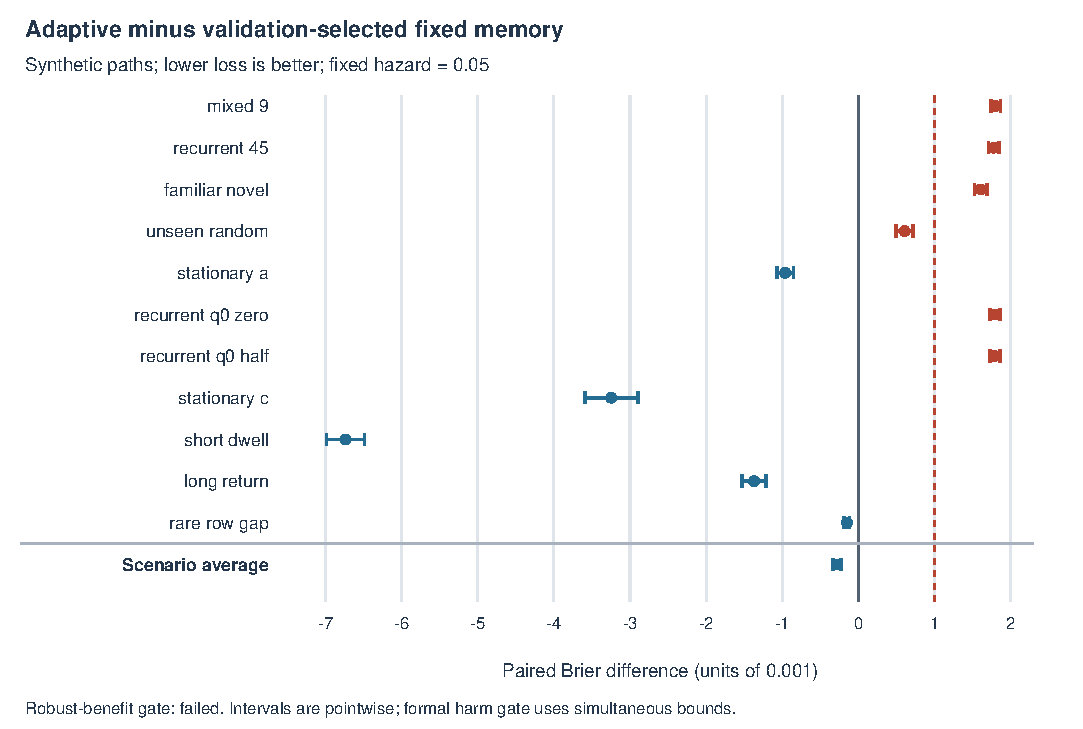
\includegraphics[width=.96\linewidth]{figures/fresh_memory_results.pdf}
\caption{Fresh computational memory evaluation. Points and bars are paired mean Brier differences and pointwise normal 95\% Monte Carlo intervals over one hundred seed clusters. Negative favors adaptive memory. The dashed $+0.001$ line shows the chosen harm margin; the formal guardrail uses separate Bonferroni upper bounds, not these pointwise bars. The overall row is the equally weighted within-seed scenario average. Known synthetic families and fresh seeds do not constitute external application validation.}
\label{fig:memory-test}
\end{figure}

All paths completed without processing or identity-assertion failures. The main adaptive and fixed arms accumulated 41.73 and 15.92 seconds respectively within an approximately 271-second evaluation, including verification overhead; this was not a resource-matched contest. Log loss, uniform mixtures, no-memory, TTL, and replacement-policy contrasts are retained as descriptive secondary results. No prompts or algorithms were tuned after outcomes.

The bounded conclusion is a small mean predictive improvement with important harms, and failure of this particular Z3 robust-benefit criterion. It does not establish equivalence, universal failure of adaptation, or a successful remedy. An amended algorithm would require a new frozen evaluation rather than reclassifying these test paths as fresh validation data.



\subsection{Quadratic portal: an independent reference also needs testing}
The unchanged inherited quadratic-portal checker executed successfully in isolation. Its analytic matching, original twenty-four-case quadrature grid, limiting checks, mixed-scalar checks, covariance fixture, and explicit negative controls passed. The new stress sweep compared the inherited energy-variable quadrature with an adaptive radial collision-flux integral over $m/T\in\{0.01,0.1,0.3,1,3,10,30,100\}$ and $rT\in\{0,10^{-6},10^{-3},0.1,1,10,50\}$: fifty-six cases spanning a wider range than the original grid.

The initial plan did \emph{not} achieve an all-pass result. Forty-seven cases met the reference-convergence and agreement criteria; nine produced adaptive-quadrature warnings. Two raw comparisons exceeded the frozen $10^{-7}$ tolerance relative to the local spectrum, with maximum discrepancy $5.65\times10^{-7}$. Because the candidate reference itself warned, this was a numerical reliability failure, not a justified rejection of the inherited formula or its physical assumptions. All initial warnings and failed flags remain in the package.

A separately frozen exploratory follow-up integrated radial momentum on intervals adapted to the oscillation phase, comparing Gauss orders 16 and 32. All fifty-six inter-order differences were below $10^{-10}$ of the local spectrum; the maximum was $5.31\times10^{-11}$. For the sixteen cases with $rT\ge10$, a distinct weighted-cosine representation gave maximum disagreement $5.45\times10^{-16}$, without warnings. Its use follows from rewriting $\operatorname{sinc}^2(kr)=[1-\cos(2kr)]/(2k^2r^2)$; it resolves an oscillatory residual rather than relying on an adaptive integral of the nearly saturated total rate.

Against the resolved reference, the largest inherited-grid discrepancy was $8.77\times10^{-8}$, and no case exceeded the original $10^{-7}$ agreement threshold. Refining the inherited energy grid in memory, without changing the physical kernel or original file, reduced the maximum discrepancy to $6.13\times10^{-15}$. The largest initial mismatch was traced to the adaptive reference; in the other threshold-exceeding case, both initial quadratures contributed comparably. This is an exploratory numerical diagnosis, not a retroactive all-pass claim for the initial protocol, and the quadrature comparison is not a rigorous error enclosure over all parameters.

Twelve additional twelve-position covariance configurations had positive minimum eigenvalues; the smallest eigenvalue normalized by the local spectrum was $0.2785$. A deliberately quarter-normalized rate disagreed with the independent normalization by $75\%$ and was detected. These tests support internal normalization and positivity on the tested fixtures. They do not establish the existence, population, temperature, or coupling of a physical scalar bath, and do not test an apparatus-specific F2 or F3 signal.

\subsection{Pure dephasing: implementation checks and informative controls}
For F1, direct exponentiation of the $4\times4$ Liouvillian was compared with the Kraus-channel expression on sixty-four seeded random density matrices, five rates, and three durations: 960 configurations. Maximum trace error was $2.22\times10^{-16}$, population change was zero to the reported floating-point precision, and maximum cross-method matrix error was $1.11\times10^{-16}$. All resulting density matrices satisfied the frozen positivity tolerance. The interference Fisher information at the stated fixture was $0.29514364485$, matching a finite-difference derivative within approximately $5.5\times10^{-12}$.

The negative-rate control produced a minimum eigenvalue of $-0.5069$ for the plus state and was correctly rejected as nonpositive. Replacing pure dephasing with amplitude damping changed a path population by $0.11050$ between the two specified rates, showing that the population-invariance check is sensitive to this different channel. Neither observation is an experimental discovery: the first is an intentionally invalid dynamics and the second a deliberately different, known channel. The tests verify implementation of the conditional statement; the physical premise that a proposed device realizes pure dephasing remains untested.

\subsection{Exact spectral response: replication and independent numerical routes}
The copied exact-mode suite was freshly executed: all 126 recorded checks passed in 54.94 seconds, and both result JSON files reproduced byte-for-byte. Forty-eight additional numerical and deliberate-control checks passed in 17.56 seconds, with no failed or inconclusive checks. The new stage uses real-axis eigenvalue fits, direct quadrature, field rescaling, projected mass calculations, and three new full external-Clifford fixtures. It reuses the original monopole matrix builder, so it is an independent numerical route for selected quantities rather than an independently rebuilt implementation of the complete model.

The real-axis fits extract $C_1$ from parallel and orthogonal quartics independently of imposing $C_0+C_1=2A_4$. The main fixture yields $C_1/C_0=1.59179263637$. Across the tested fit ranges and angular cutoffs, the maximum coefficient discrepancy from the reference is $3.38\times10^{-11}$ and the maximum protected-sum residual is $3.49\times10^{-11}$, below the frozen $10^{-9}$ and $10^{-10}$ tolerances respectively. This addresses the principal T1 distinction between unequal exact mixed quartics and the equal local approximation.

Direct quadrature gives the profile difference $\Delta G=1.8962286435064\times10^{-9}$ at both tested cutoff/order combinations. For the T2 field-scaling diagnostic, halving the field scale produces remainder ratios $0.06258796$ and $0.06252199$, near the quartic reference $1/16=0.0625$. The maximum normalized photon-null residual is $1.93\times10^{-12}$, the largest independent Ward discrepancy is $1.33\times10^{-12}$, and the largest discrepancy among three new full-Clifford fixtures is $7.68\times10^{-14}$.

Four controls were detected: imposing the local quartic equality, changing the parallel Yukawa coupling, using a nonneutral photon generator, and omitting the Pauli vertex. They demonstrate sensitivity to those specific violations, not to every possible error. All seventy-six original source files checked by this workstream and all fourteen frozen files remained unchanged. Finite cutoffs, double precision, shared building blocks, and a limited set of fields restrict the result. No coupled vacuum, higher-dimensional anomaly completion, threshold-matched particle spectrum, pole mass, observed coupling, or physical field was established. T3 and the empirical portion of T4 therefore remain open.

\subsection{Which prediction targets were actually tested?}
\begin{longtable}{@{}>{\raggedright\arraybackslash}p{.11\linewidth}>{\raggedright\arraybackslash}p{.40\linewidth}>{\raggedright\arraybackslash}p{.42\linewidth}@{}}
\toprule
Cards & Executed scope & Remaining interpretation boundary\\\midrule
\endfirsthead
\toprule Cards & Executed scope & Remaining interpretation boundary\\\midrule\endhead
\bottomrule\endfoot
Z1 & Revised-system software and synthetic challenge; no original-versus-revised factorial. & The causal contribution of the relation schema remains untested.\\
Z2 & Revised single pass versus blind three-role system on the same new cases. & No blind-versus-informed challenger arm, matched coverage, or matched resource budget; no general role-superiority claim.\\
Z3 & Frozen adaptive-versus-validation-selected-fixed comparison on fresh paths. & Joint minimum-effect and robustness criterion failed; transfer beyond known generators remains untested.\\
Z4 & Integrity controls and synthetic stale/dependent/conflicting-evidence cases. & No metadata-ablation factorial or independent human labels; semantic provenance benefit not causally isolated.\\
F1 & Liouvillian/Kraus agreement and population/readout controls. & Conditional implementation result, not evidence that a device realizes this channel.\\
F2 & Wider numerical kernel sweep and exploratory quadrature diagnosis. & No prepared bath or measured interferometric visibility; physical shape prediction untested.\\
F3--F4 & Algebra retained; no new cross-channel fit or calibrated source-factorial observation. & Physical sources, nuisance likelihoods, and observational identifiability remain open.\\
T1--T2 & Fresh suite plus real-axis, quadrature, field-scaling, null/Ward, and control tests. & Selected finite numerical checks pass; shared builder and truncated model limit independence.\\
T3--T4 & No new coupled-vacuum solution, anomaly completion, or measured running fit. & Physical consistency/comparison gates remain unresolved.\\
\end{longtable}


\subsection{Reproducibility and boundaries of the resulting claims}
The local test bundle preserves protocols, source and code hashes, environments, exact commands, raw outcomes, warnings, negative controls, and summary statistics. Frozen files are checked after execution. Earlier computational artifacts remain separately identifiable, and the version 2 manuscript is preserved alongside the current version. New test counts and rates are not combined into a single success score because the units and inferential targets differ.

The defensible advancement is more specific than general model validation: numerical routes agree on selected conditional physical coefficients; implementation checks detect defined violations; a wider portal sweep exposes and diagnoses a reference-integrator limitation; and new algorithm evaluations quantify behavior on constructed tasks. Whether a source exists in nature, whether an apparatus realizes the assumed channel, and whether a proposed completion matches observed matter require physical evidence that this local campaign does not supply.
